\pagestyle{fancy}
%%%%%%%%%%%%%%%%% KOS reconstruction


In this chapter, the application of the ML algorithms for optimizing \PKshort reconstruction (and thus proper identification) will be discussed. As opposed to the traditional method mentioned in the chapter before, the predicted advantages and disadvantages are presented in the table below:
\begin{table}[H]
    \begin{tabular}{|l|l}
    \hline
    \multicolumn{1}{|c|}{\textbf{Advantages}}        & \multicolumn{1}{c|}{\textbf{Disadvantages}}    \\ \hline
    Non-linear in multi-dimensional space            & \multicolumn{1}{l|}{Not easily interpretable}  \\ \hline
    Automatization of the selection process          & \multicolumn{1}{l|}{Computationally expensive} \\ \hline
    Partially collision simulating model-independent &                                                \\ \cline{1-1}
    \begin{tabular}[c]{@{}l@{}}With \emph{probability} a  value from which we consider \\a particle as a K-short particle can be chosen;\\ it can aim for better reconstruction efficiency \\ or a better background reduction\end{tabular} &
       \\ \cline{1-1}
    \end{tabular}
\caption{\label{tab:mlselection}Advantages and disadvantages of ML selection criteria optimization}
\end{table}
\\The accuracy of these predictions will be checked in this chapter. The results of the K-short reconstruction optimization and has been presented before in \cite{get involved} (some fragments of this report will be presented in the following sections).

\section{Model preparation}\thispagestyle{fancy}
All the data is stored in the AnalysisTree format, later passed through the PFSimple (C++ with ROOT framework),  which returns all the possible K-short's daughter particles pairs, from which we could reconstruct a K-short particle. All the possible pairs along with the variables (described in the chapter before) are available for training in the \emph{PlainTree} format, which can be loaded into Pandas Dataframe (Python), using a function prepared by the CBM-ML group\cite{plaintree}. Version 3.7 of Python was used, with the following libraries:
\begin{itemize}
    \item pandas (version 1.3.4)
    \item xgboost (version 1.3.3)
    \item scikit-learn (version 1.0.1)
    \item bayesian-optimization (version 1.1.0)
\end{itemize}
The parts of the code used for the ML model training are shown in the appendix A.

\subsection{Data enriching}
There are two problems to tackle before providing datasets to our ML model: underrepresentation and dependence of collision simulation model.

%---------------dependence of collision simulation model
\subsubsection{Dependence of collision simulation model}
To make the ML model partially independent of the collision simulation model,  select:
\begin{itemize}
    \item primary Ks candidates only in 5$\sigma$ region: $0.43485 - 0.56135$ (GeV/$c^2$) from DCM-QGSM-SMM model, (simulation data)
    \item background outside 5$\sigma$ region from UrQMD model, which mimics experimental data (will be replaced by real experimental data while CBM experiment starts)
\end{itemize}
Also, the UrQMD model is being used as a test dataset (as the model does not "know" the signal candidates from this MC model).
\begin{figure}[H]
    \centering
    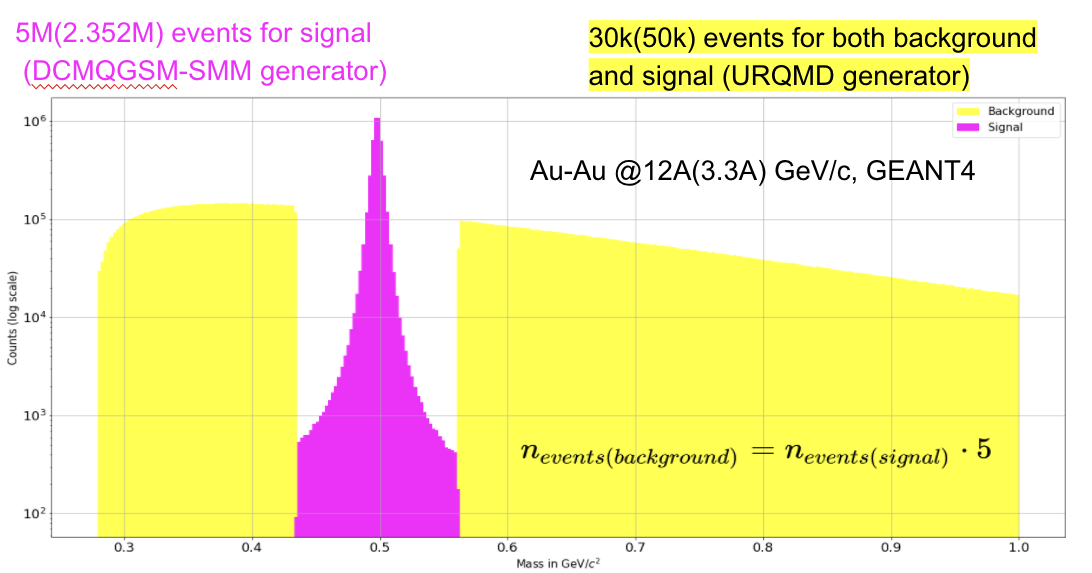
\includegraphics[width=1\textwidth]{img/dataset.png}
    \caption{Data enriching}
\end{figure}
In total, the following datasets will be used:
\begin{itemize}
    \item 5M (2.352M) events for signal generated in DCM-QGSM-SMM
    \item 30k(50k) events for both background and test dataset generated in UrQMD
\end{itemize}
Au-Au @12A(3.3A) GeV/c passed through CBM setup in GEANT4, and PFSimple.


%---------------underrepresentation
\subsubsection{Underrepresentation}
As in the simulated data, less than 0.1\% of K-short candidates are signal candidates, the ratio in the training dataset has to be changed so that the model learns how to identify signal candidates well. The number of background entries is rescaled by this formula:
\begin{equation}
    n_\text{events(background)} = 5 \cdot n_\text{events(signal)}
\end{equation}


%------------- data cleaning
\subsection{Data cleaning}
To reject the numeric values of parameters which do not have physical sense, but are present in the data set, some selection criteria are applied before the beginning of the model training. Similarly, we some values which might be possible but are rare enough are rejected, to reduce the amount of data.

%----------------------- Invariant mass
\subsubsection{Invariant mass}
As the K-short particle decays into two pions, its invariant mass cannot be smaller than the mass of the two pions, so:
\begin{center}
    $m_\text{inv} >$ 0.279 GeV/$c^2$
\end{center}
Also, to reduce the amount of data:
\begin{center}
   $m_\text{inv} <$ 1 GeV/$c^2$
\end{center}

%---------------- distances
\subsubsection{Distances and \emph{x, y, z} coordinates}
Distance between the primary vertex (the point where the collision of the nuclei happens), and the secondary vertex (the extrapolated point where the two daughter particles should have crossed each other)  - $l$ and the distance of closest approach between the two pions - $DCA$ - should not be smaller than zero:
\begin{center}
    $DCA$, $l$, $\frac{l}{\Delta l}$ $> 0$
\end{center}

Also, due to the sizes of the tracking system (the largest station has an area of 1m$^2$):
\begin{center}
    $DCA < 100 $ cm
\end{center}
For the same reason:
\begin{center}
    $|x|, |y| < 50$ cm
\end{center}
As the particle has to hit 3 stations of the tracking system, and the last two are placed above 80 cm:
\begin{center}
    $l < 80$cm
\end{center}
For the same reason, and because of the fixed target geometry of the detector:
\begin{center}
    $-1$ cm $< z < 80$ cm
\end{center}
To reduce the data, we set:
\begin{center}
    $\frac{l}{\Delta l} < 15000$
\end{center}
However, in the KFParticle package $l$ is assumed to be signed by design, and one can notice that actually, some data entries have a negative value of distance, for both signal and background. As the \emph{quality cuts} should be rather conservative, the following ranges are set:
\begin{center}
     $l >$ -5 (cm)\\
     $\frac{l}{\Delta l} >$ -25
\end{center}
%----------------- momentums
\subsubsection{Momentums}
The fixed target geometry of the detector requires that:
\begin{center}
    $p_Z > 0 $ GeV/c
\end{center}
To reduce the data:
\begin{center}
    $p < 20$ GeV/c; $p_T < 3$ GeV/c
\end{center}


%-------------- chi square
\subsubsection{Chi square}
Since $\chi^2$ is a squared distance, all the values must be larger than zero:
\begin{center}
    $\chi^2 > 0$
\end{center}
To reduce the data, following the maximal values are selected:
\begin{itemize}
    \item $\chi^2$ first and second $< 3 \cdot 10^7$
    \item $\chi^2_{geo} < 10000$
    \item $\chi^2_{topo} < 100000$
\end{itemize}

%----------------------- pseudorapidity
\subsubsection{Pseudorapidity}
As pseudorapidity depends on polar angle as $\eta = -\ln{\tan(\frac{\theta}{2})}$, and the STS covers the polar angles between 2.5$^{\circ}$ and 25$^{\circ}$, for which the pseudorapidity values would equal:
\begin{center}
    $ 1.5< \eta < 3.82 $
\end{center}
However, due to the magnetic field, the pseudorapidity is constrained to following values:
\begin{center}
    $ 1.0< \eta < 6.5 $
\end{center}
with which we loose 0.06\% of data for signal (instead of 5.66\%) and 0.08\% of data for background (instead of 6.75\%)

%------------------ variables selection
\subsection{Variables selection}
The last step before training our model is the selection of variables which will be used in the training of the discriminator. To make the model simpler, there is no need to use two variables if they are strongly correlated with each other. Also, to avoid signal/background classification directly by invariant mass, variables strongly correlated with the invariant mass of background should be omitted.
\subsubsection{Correlation matrix}
The Pearson correlation efficient of each variable is being calculated following this formula:
\begin{equation}
    \rho = \frac{\operatorname{COV}(X, Y)}{\sigma_X \times \sigma_Y}
\end{equation}
where:
\begin{equation}
    \operatorname{COV(X, Y)} = \operatorname{E}\left[\left(X - \operatorname{E}\left[X\right]\right) \left(Y - \operatorname{E}\left[Y\right]\right)\right]
\end{equation}
\begin{equation}
    \sigma_X = \sqrt{\operatorname{E}\left[\left(X - \operatorname{E}\left[X\right]\right)^2\right]}
    \label{stddev}
\end{equation}
They are then plotted in a matrix:
\begin{figure}[h!]
    \centering
    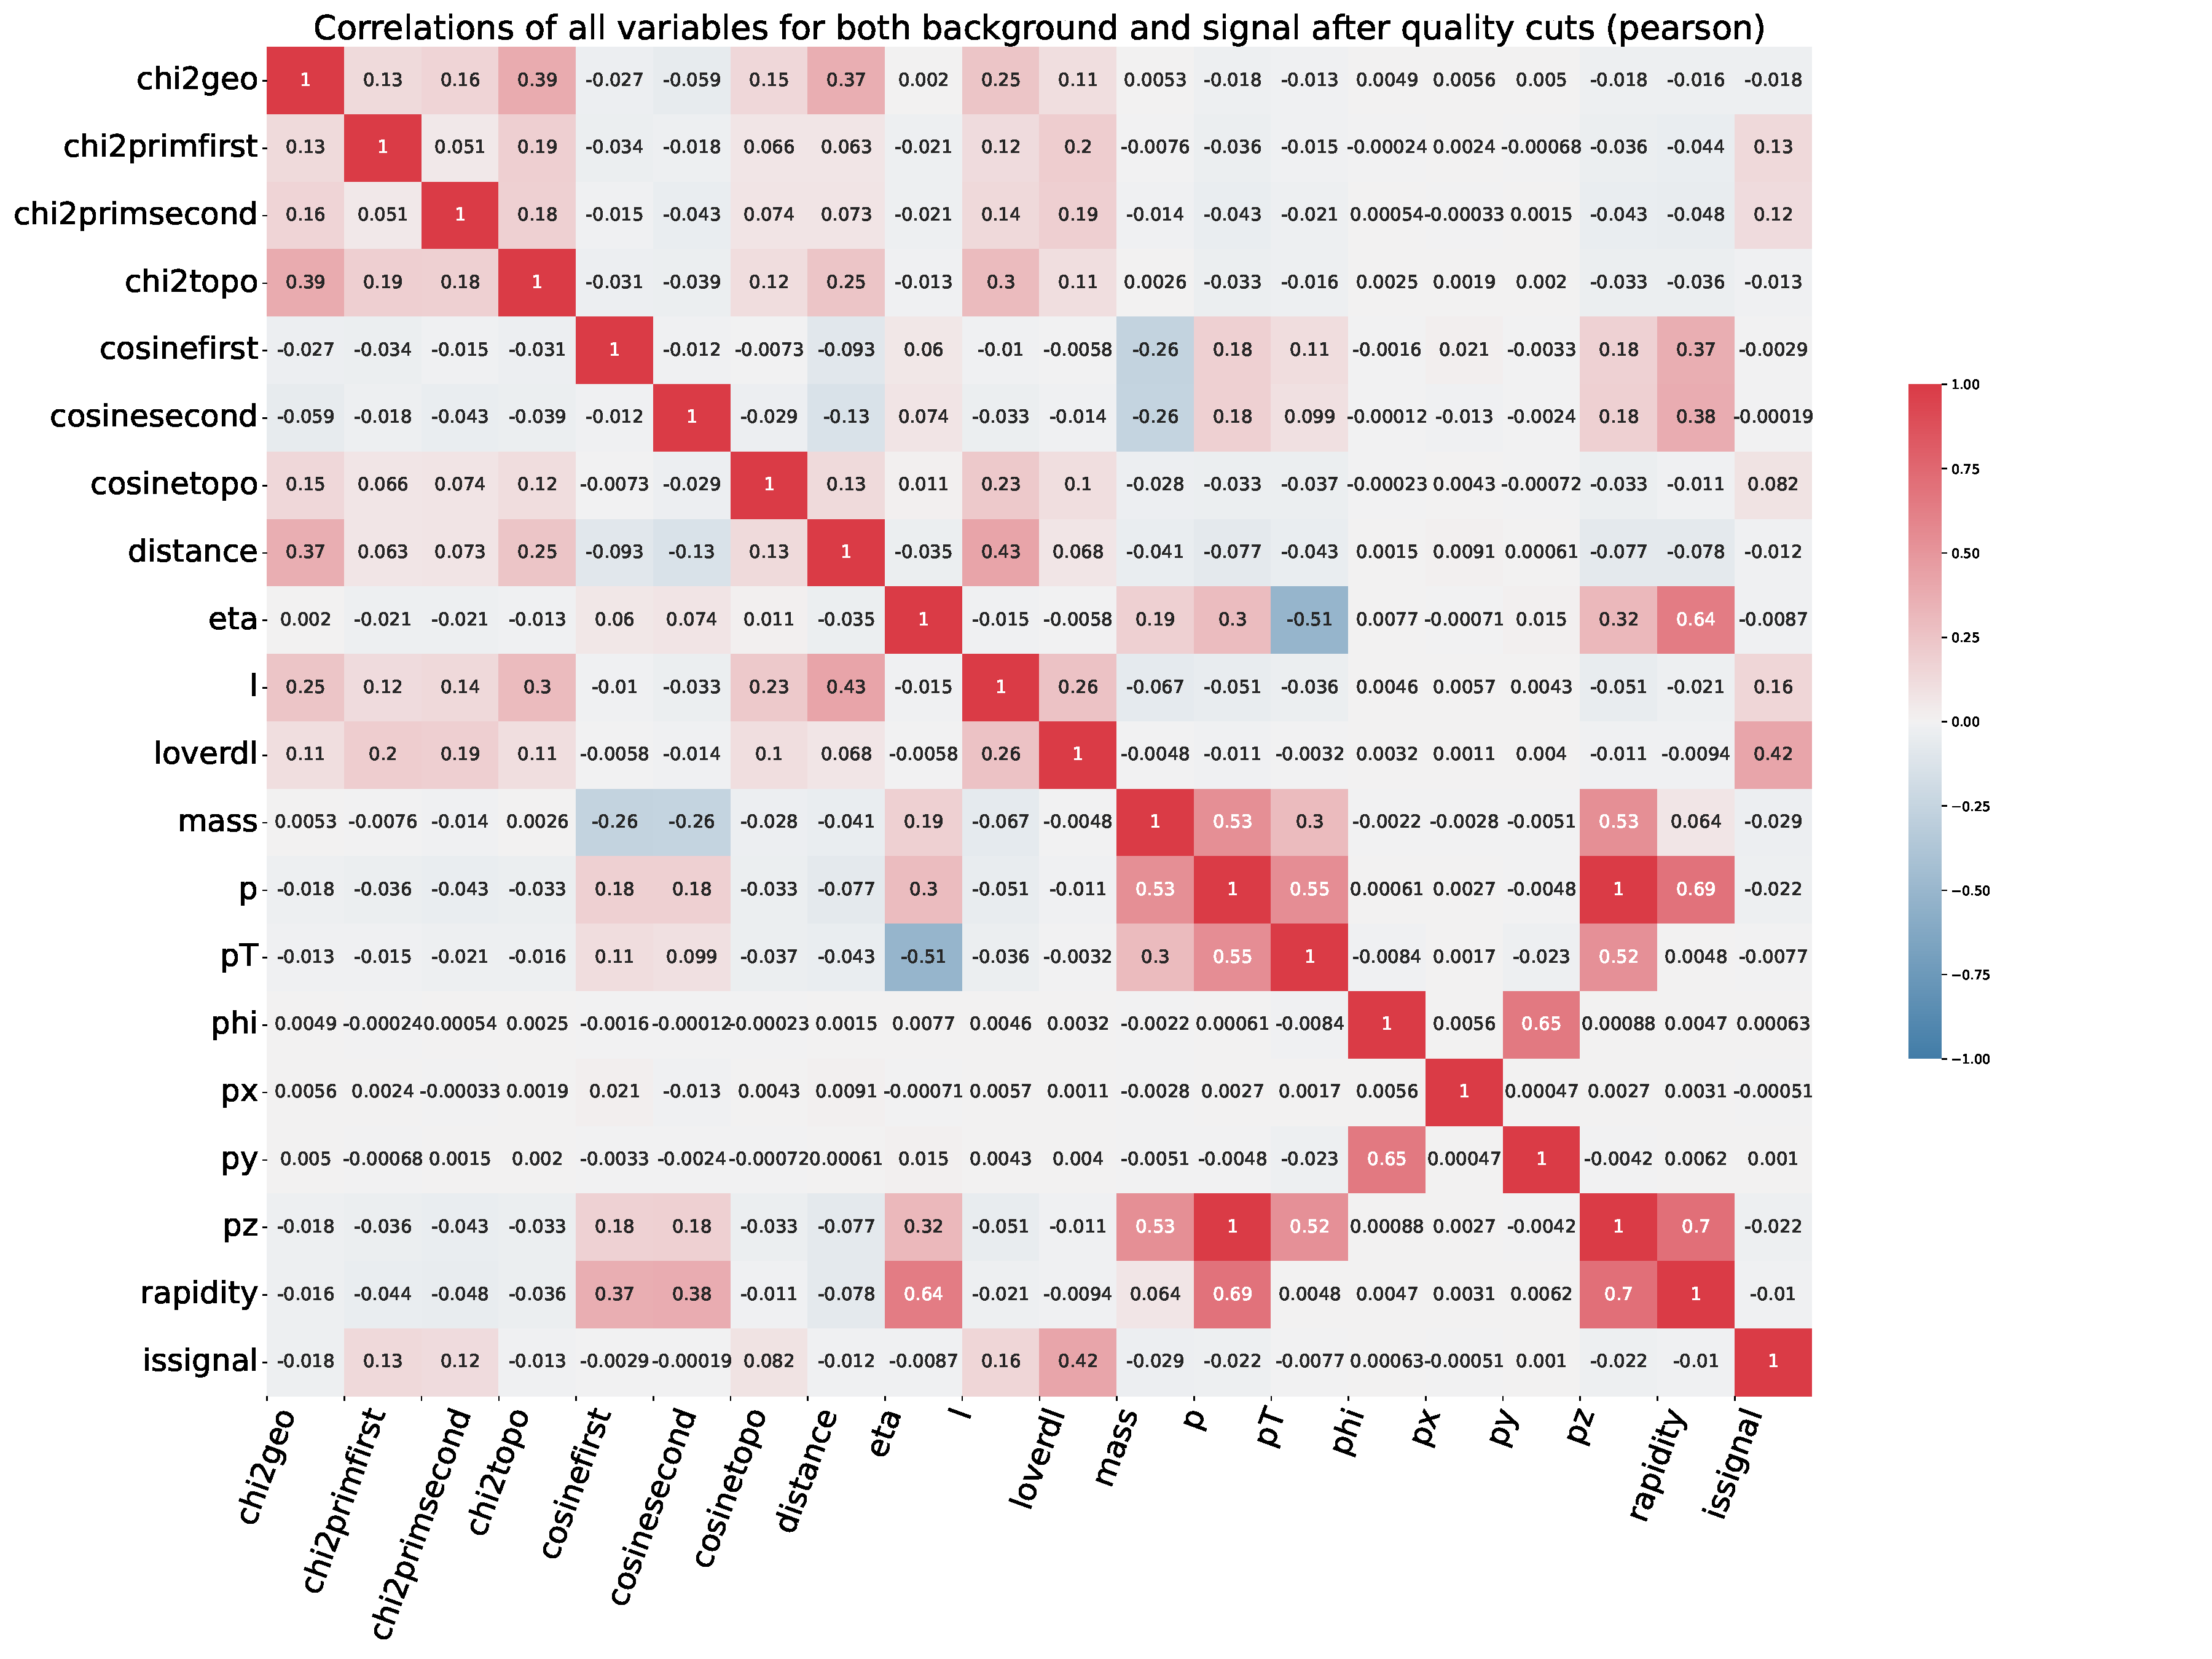
\includegraphics[width=1.1\textwidth]{img/Correlations_of_all_variables_for_both_background_and_signal_after_quality_cuts_(pearson).pdf}
    \caption{Correlation matrix}
\end{figure}
\clearpage
%-------------------- Correlation with invariant mass
\subsubsection{Correlation with invariant mass}
Later, the correlation (Pearson coefficient) of each variable with the invariant mass of (separately) signal and background is being checked 
\begin{figure}[H]
    \centering
    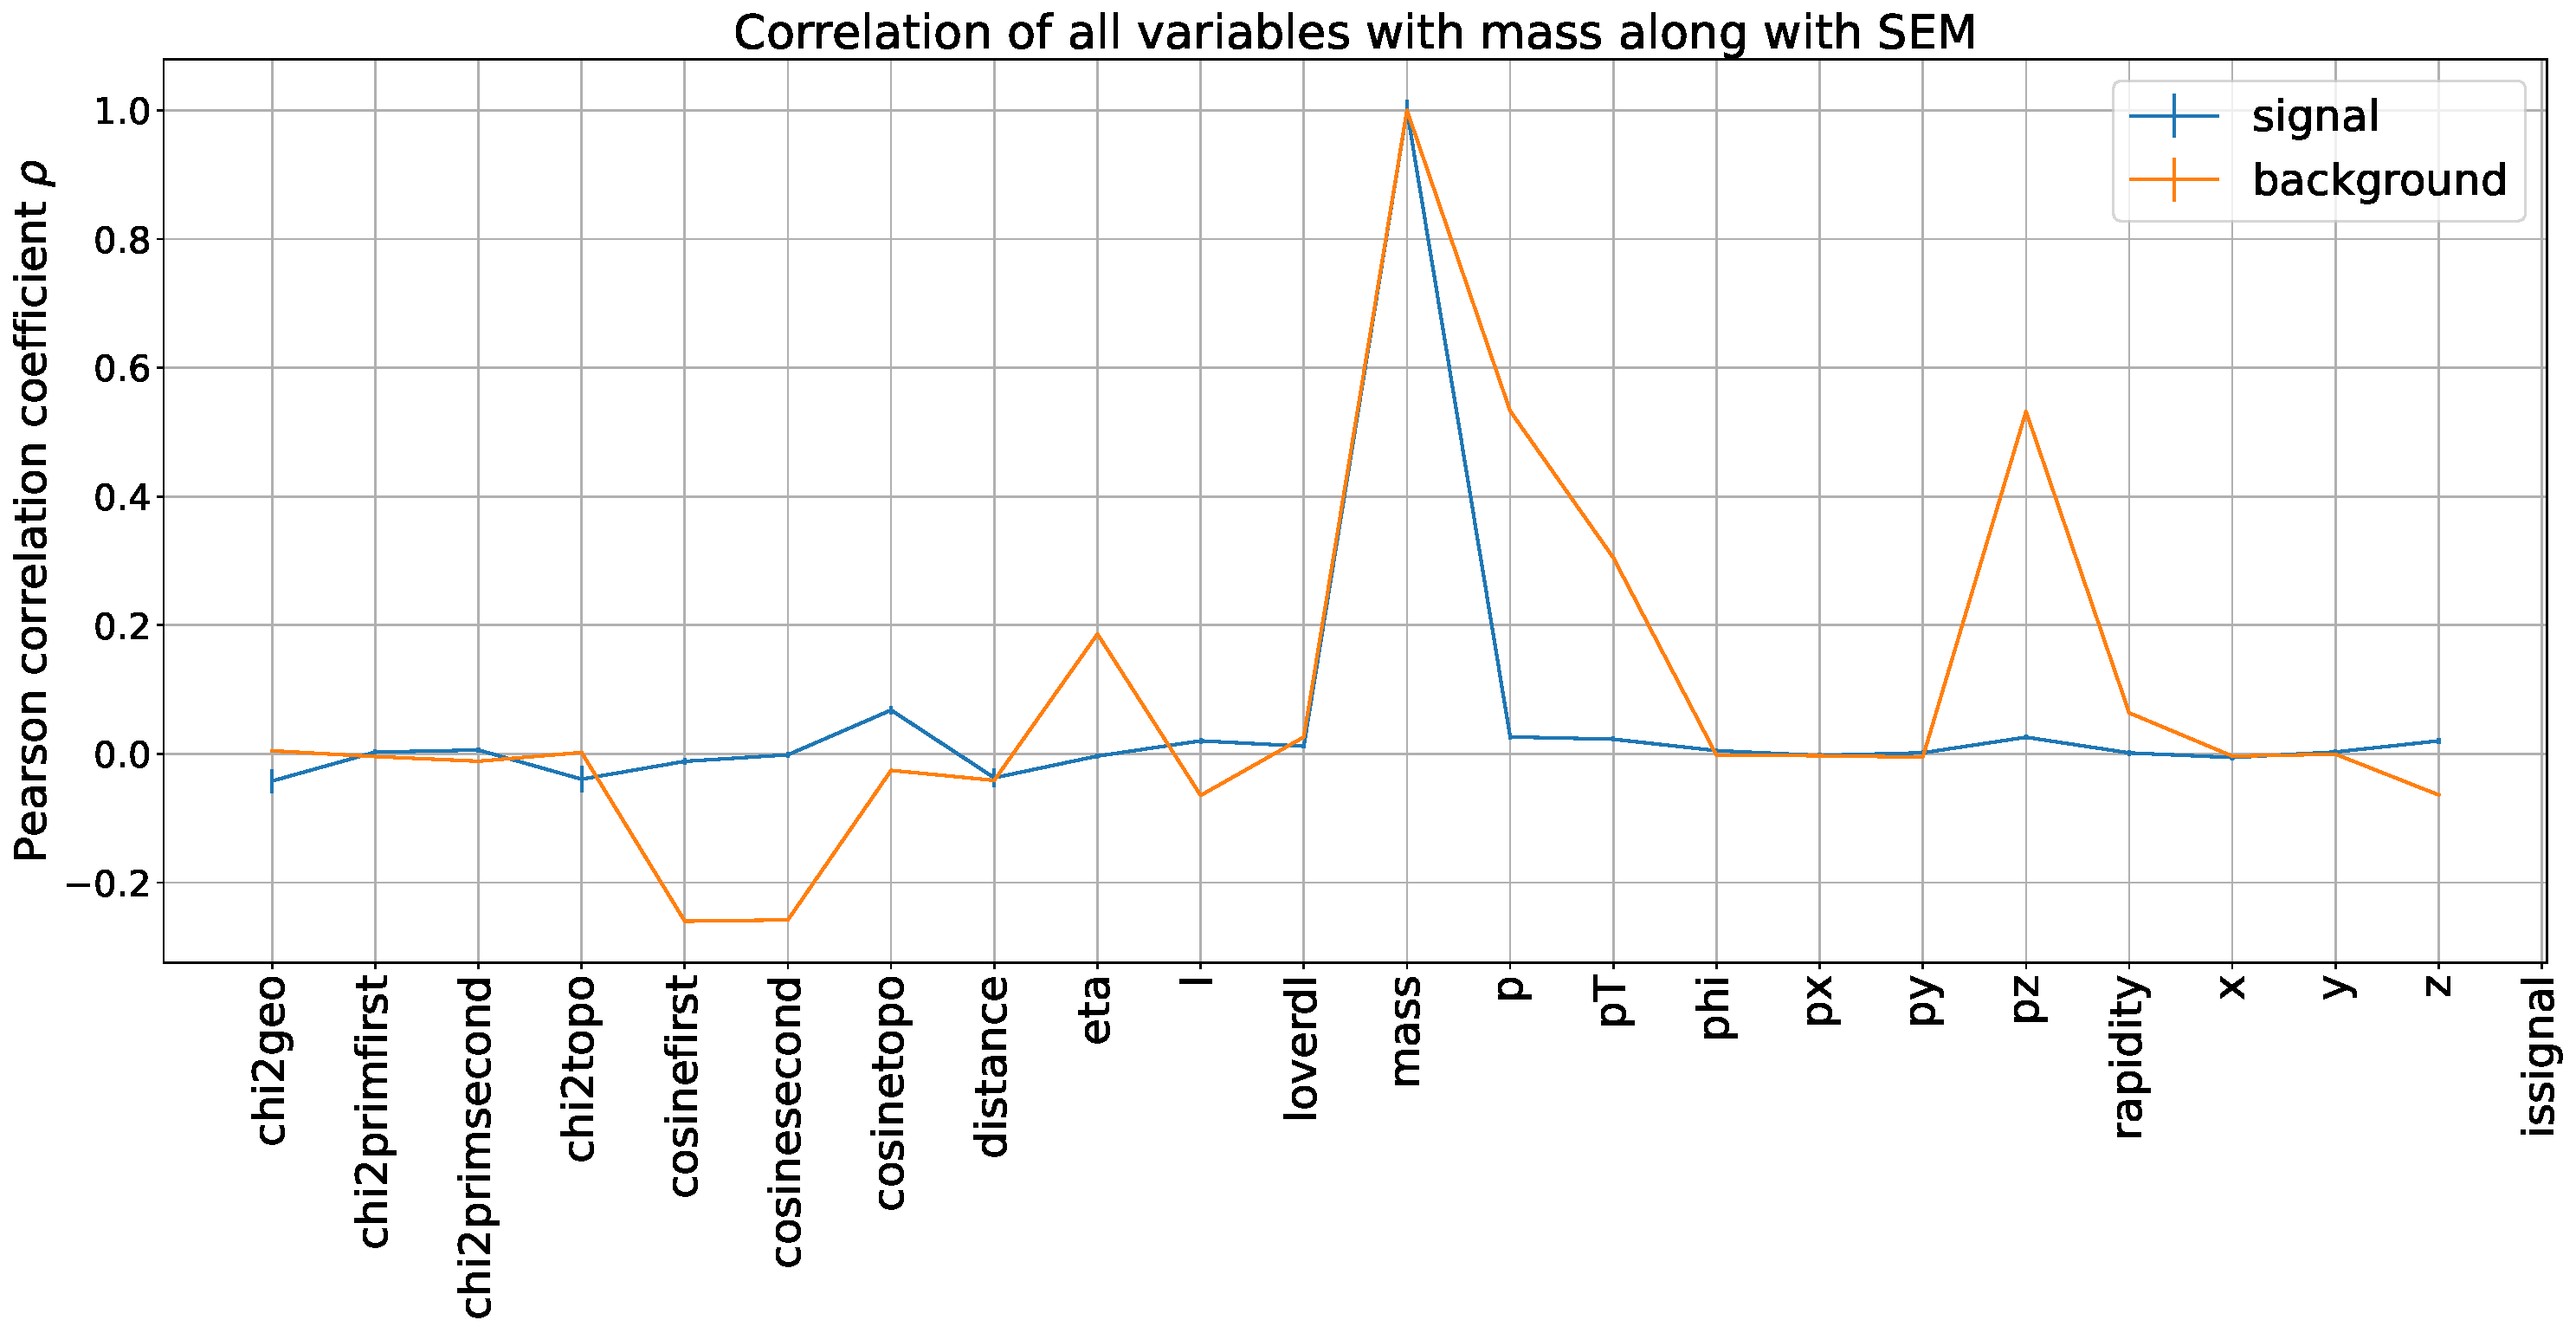
\includegraphics[width=1\textwidth]{img/Correlation_of_all_variables_with_mass_along_with_SEM.pdf}
    \caption{Correlation of all variables with mass}
\end{figure}

%-------------------- Selected variables
\subsubsection{Selected variables}
Based on that, the following 6 variables are selected for the training: $L/\Delta L$, $DCA$;  $\chi^2_{geo}$, $\chi^2_{topo}$, $\chi^2_{prim first}$, $\chi^2_{prim second}$

%----------------------- Model training
\section{Model training}
%--------- results for 12A GeV/c
\subsection{Results for $p_{\text{beam}}$ = 12A GeV/c}
Having prepared the data, the training of the ML algorithm may be initiated. To choose the hyper-parameters of the XGBoost model, the Bayesian Optimisation package was used.\\
%--------------- Cross validation
\subsubsection{Cross validation}
To check if the model works as well on new data, as on the training dataset,  Receiver Operating Characteristic and probability plot are prepared.

Receiver Operating Characteristic illustrates the diagnostic ability of a binary classifier. Threshold on the ROC (Receiver Operating Characteristic) curve which maximizes Approximate Median Significance 
\begin{equation}
    \text{AMS}= \sqrt{2} [(tpr + fpr) \log(1 + tpr/fpr) - tpr]
\end{equation}
(where $t(f)pr$ is true (false) positive rate) on the test sample is the best threshold.
\begin{figure}[H]
    \centering
    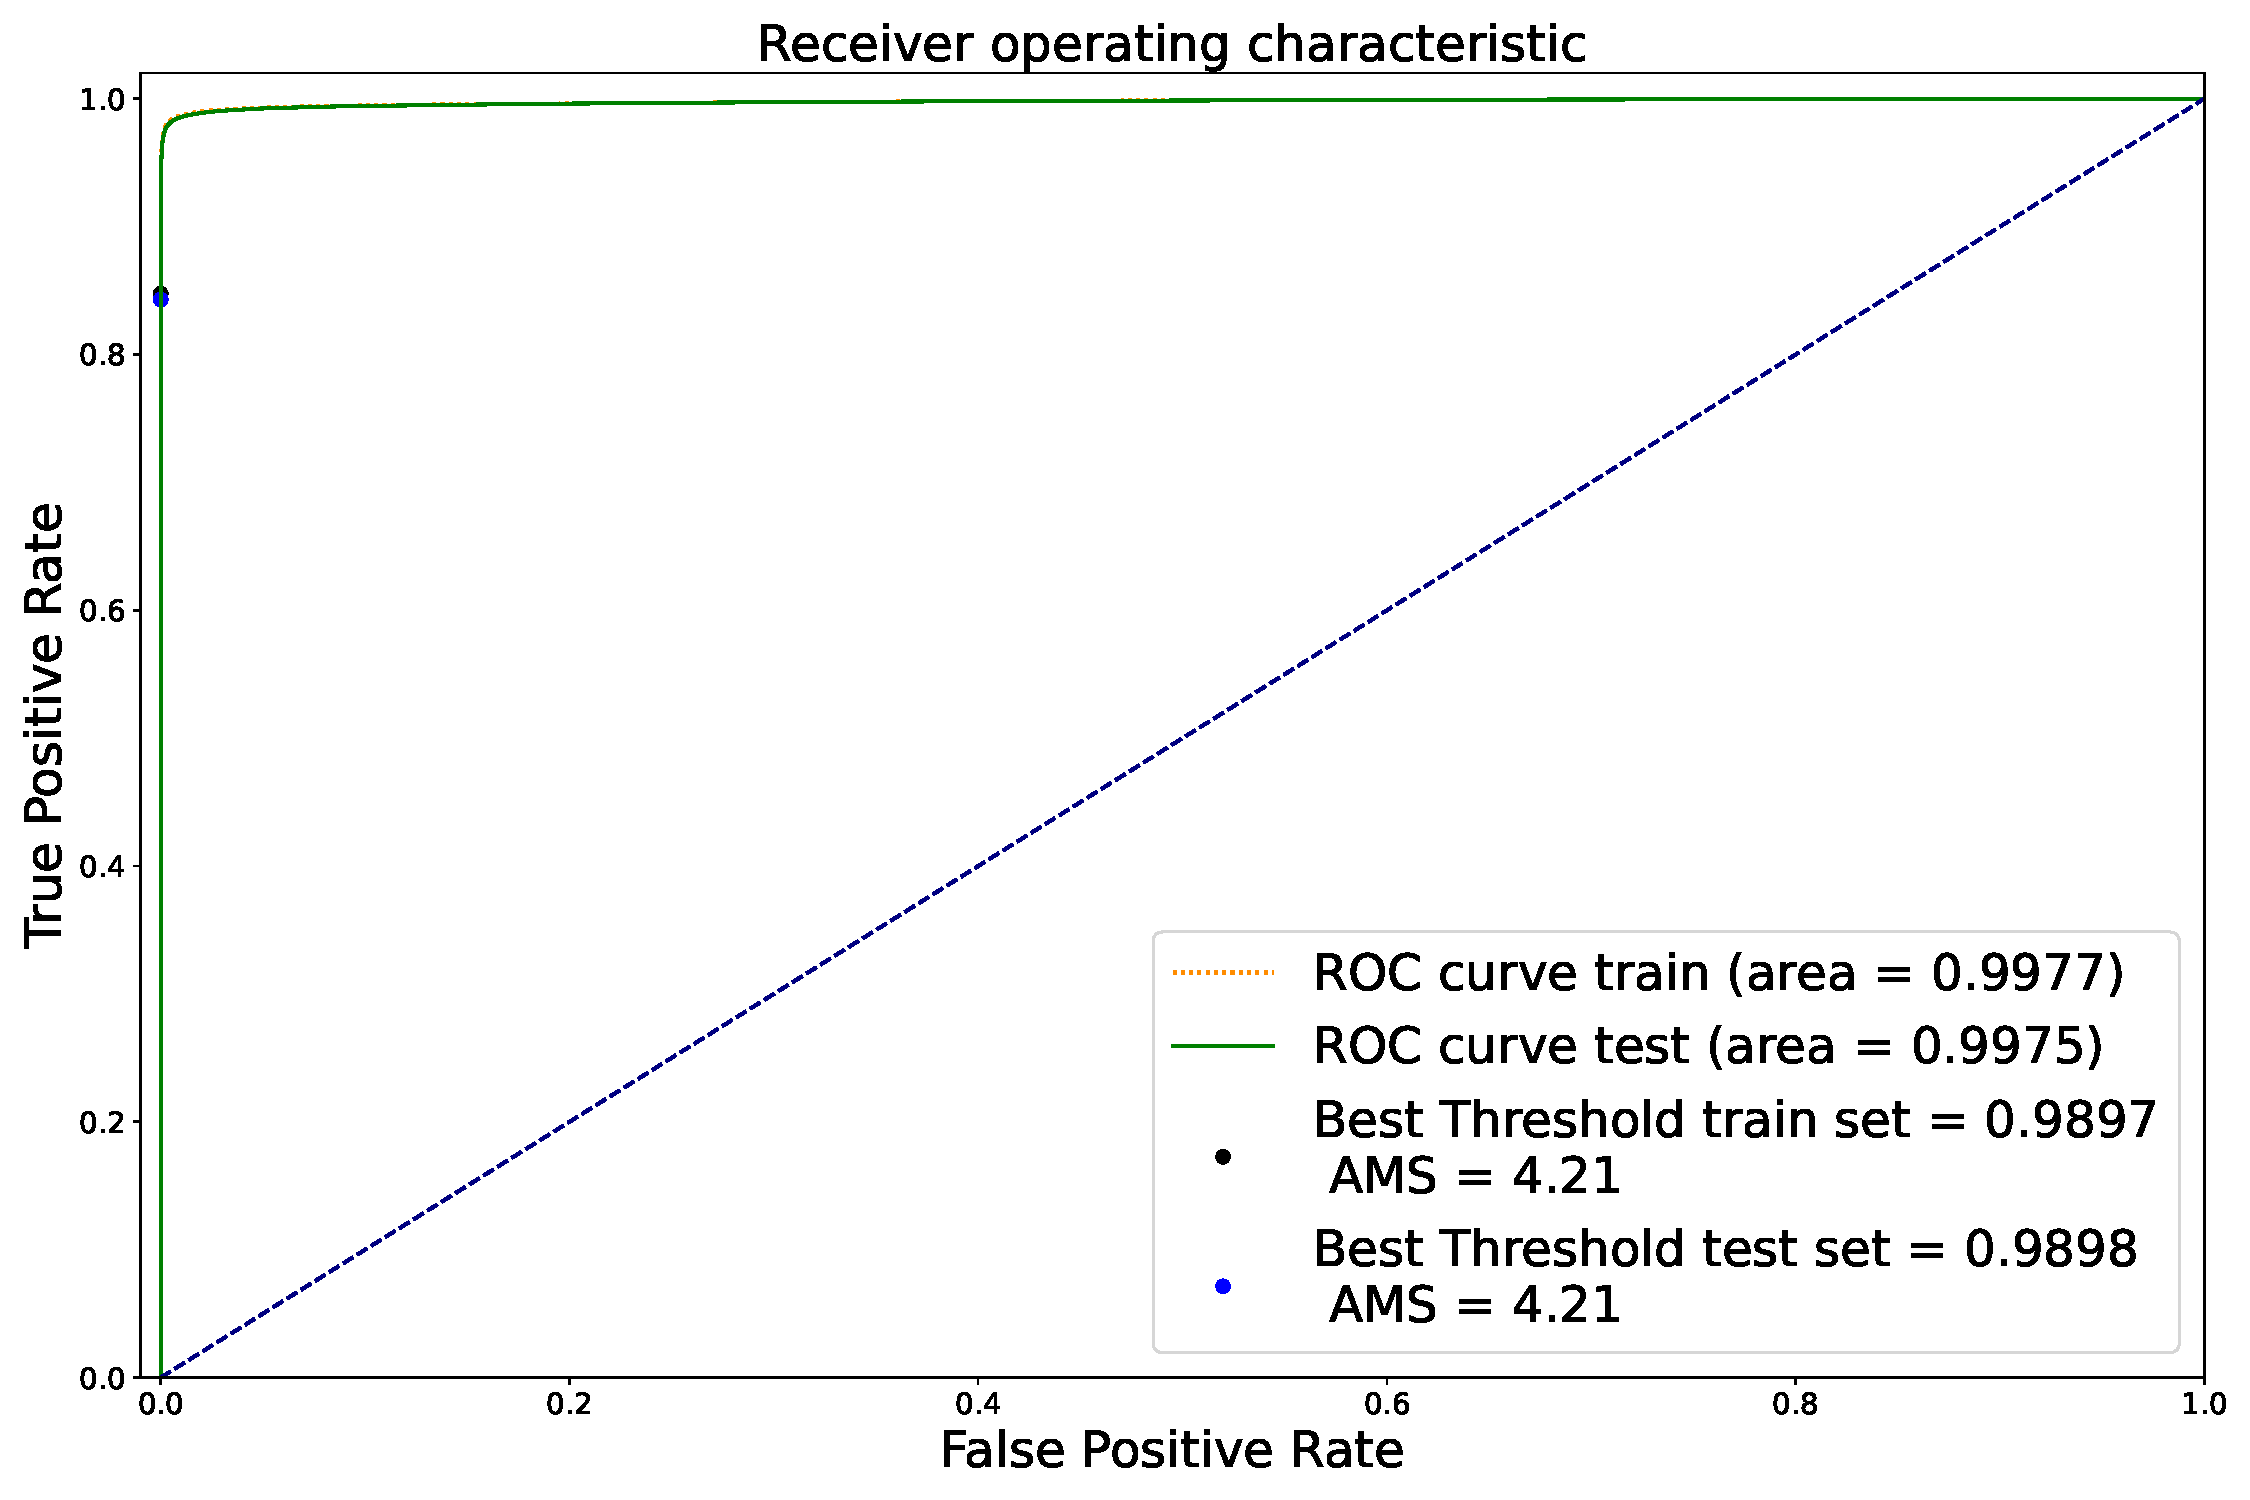
\includegraphics[width=1\textwidth]{img/ams.pdf}
    \caption{Receiver Operating Characteristic}
\end{figure}
We see that the optimal point on ROC is similar for both train and test datasets.
The graph of signal/background share in both train and test datasets is also plotted.
\begin{figure}[H]
    \centering
    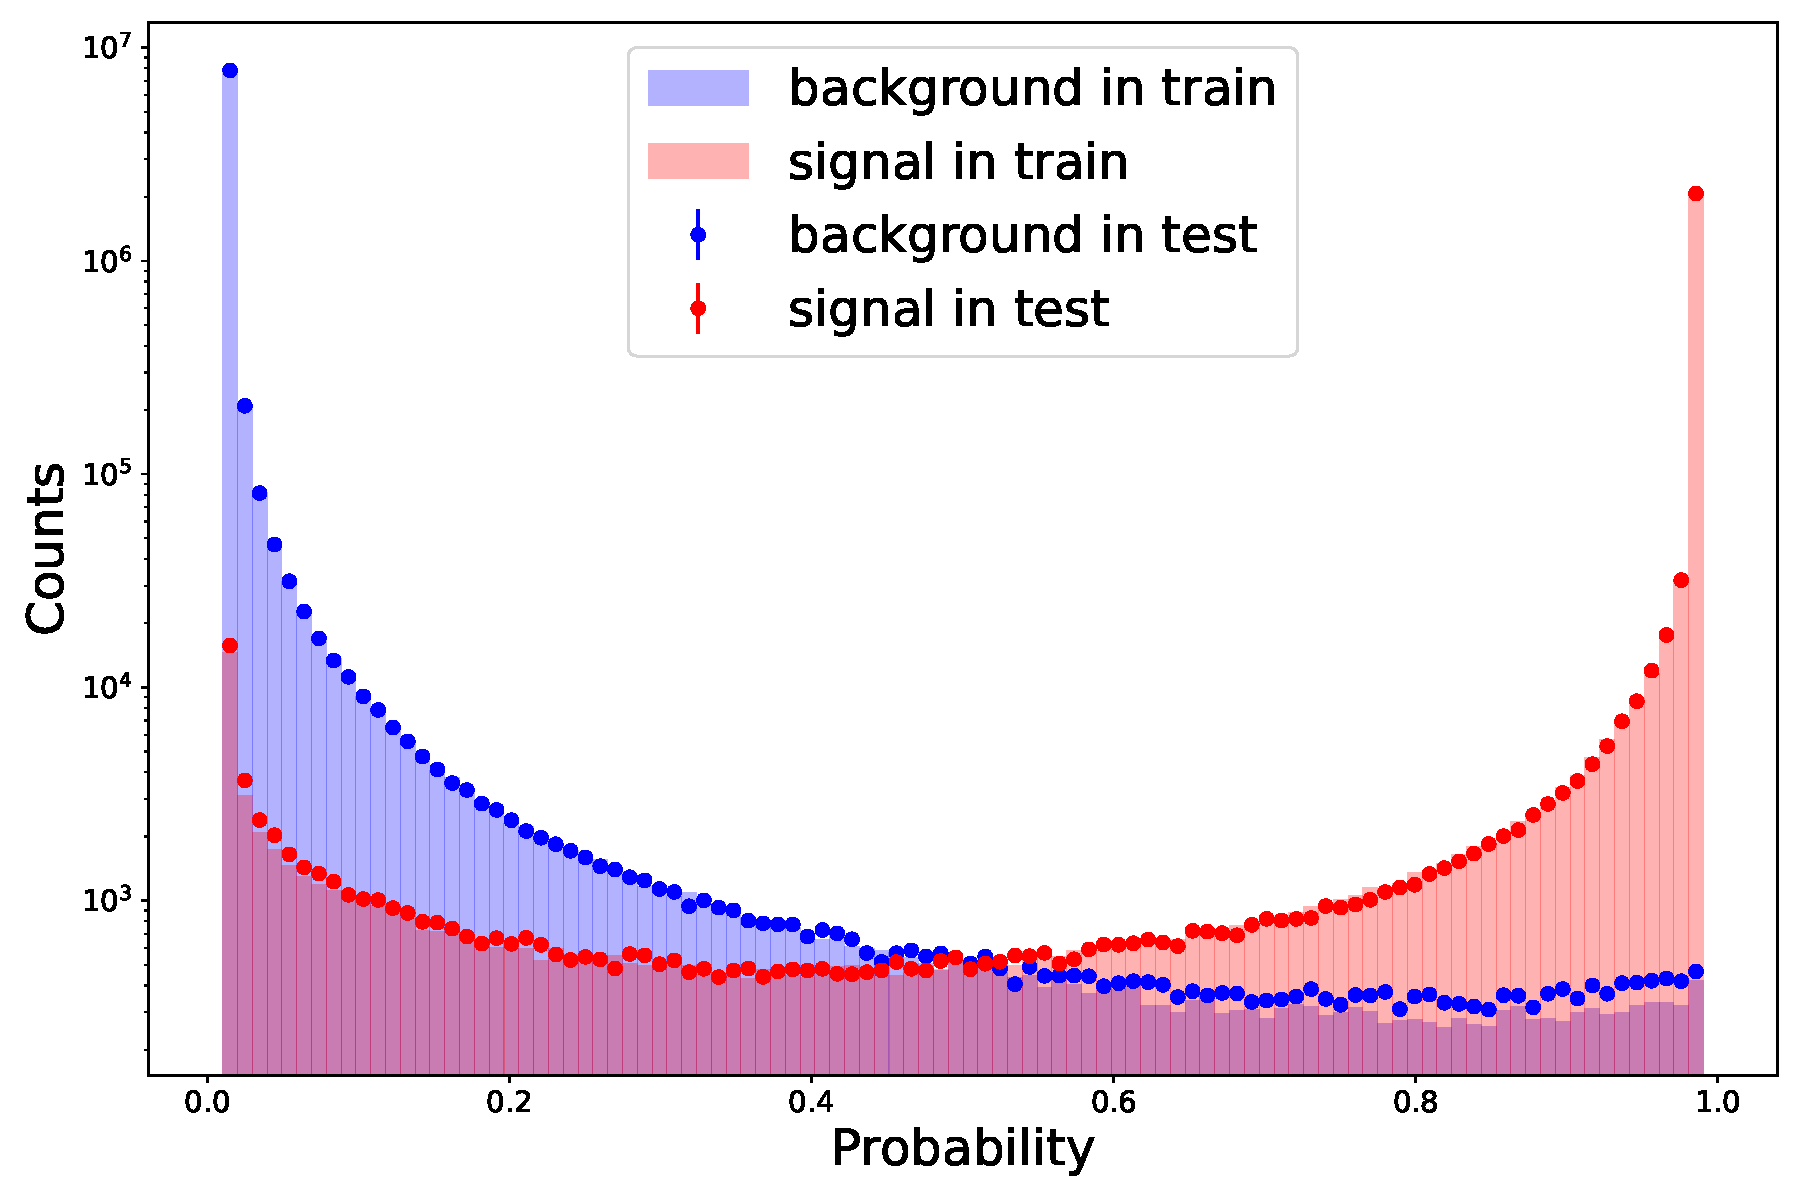
\includegraphics[width=.8\textwidth]{img/probability.pdf}
    \caption{Probability plot}
\end{figure}

Once again, the results are similar for the two datasets. Hence, we can say that our model is not overtrained (works well on new data).

The invariant mass distribution before and after XGB selection is presented before:
\begin{figure}[h!]
    \centering
    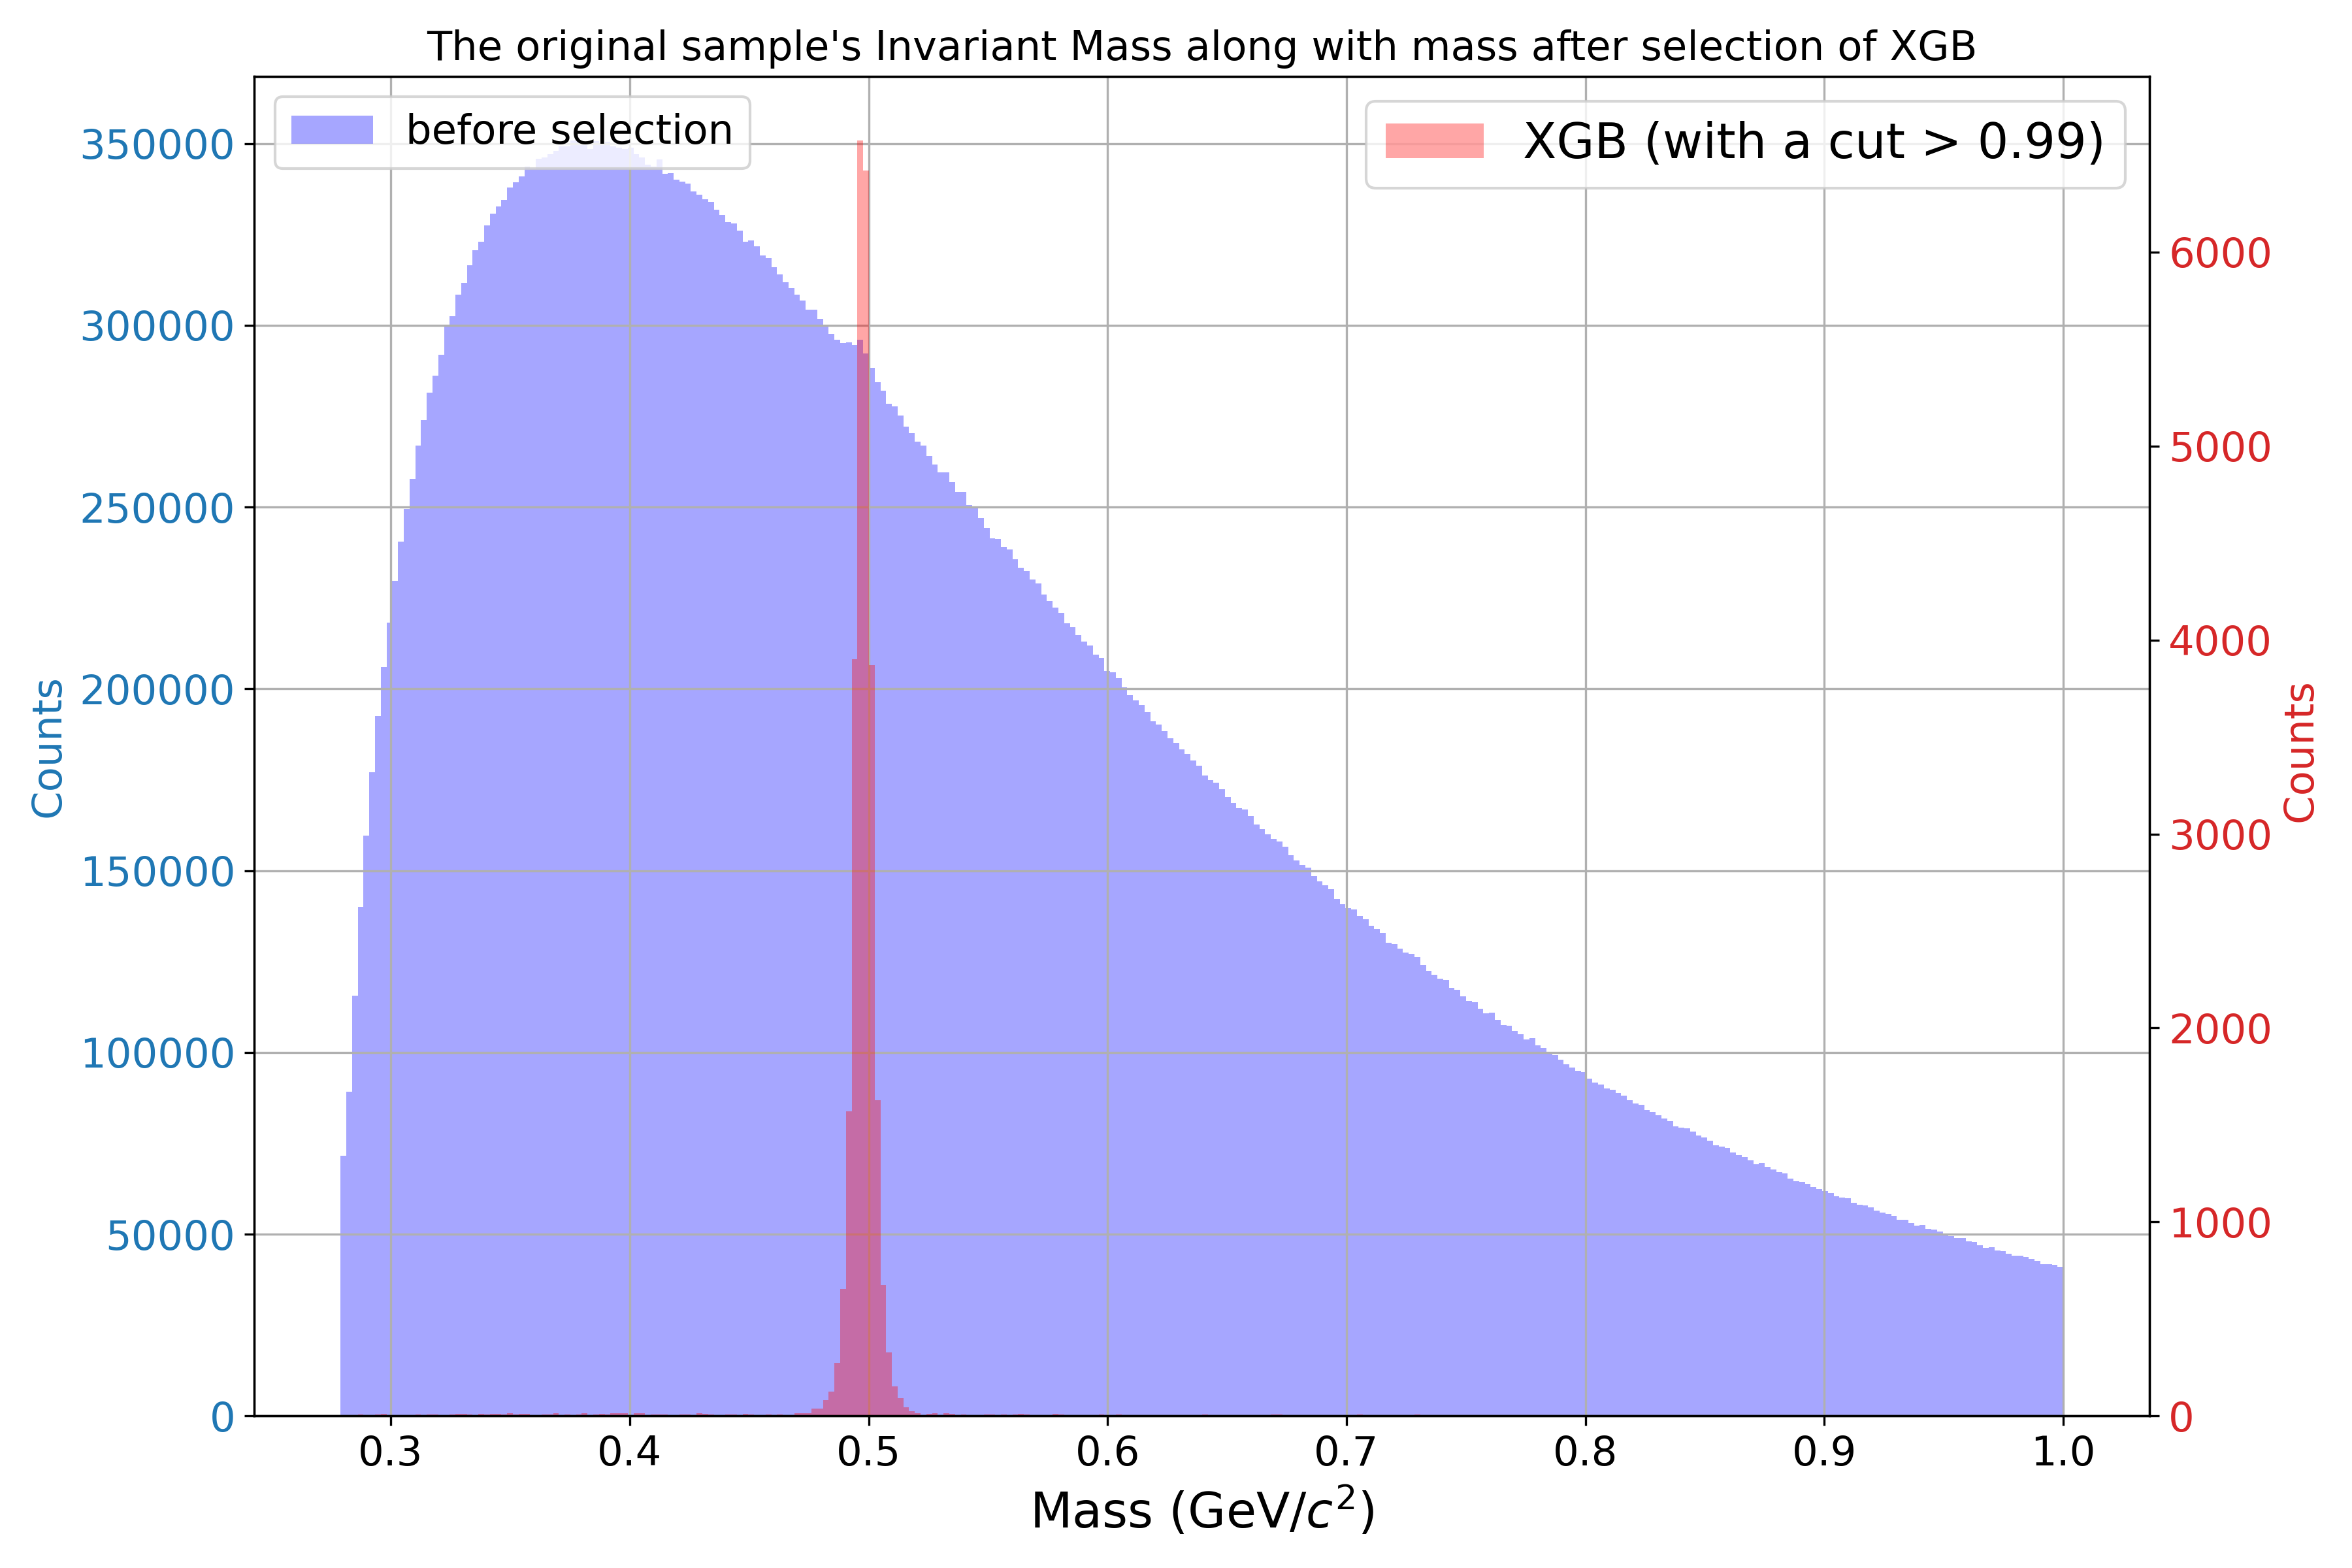
\includegraphics[width=.9\textwidth]{img/cut_visualization.png}
    \caption{Invariant mass distribution}
\end{figure}


%--------------- Comparison with default KFPF Cuts
\subsubsection{Comparison with default KFPF Cuts}
KFParticleFinder has default selection criteria, which can be compared with ML selection:
\begin{itemize}
    \item $L/\Delta L > 5 $
    \item $DCA < 1 $ cm
    \item $\chi^2_{geo} < 3 $
    \item $\chi^2_{prim} > 18.4 $
    \item $\cos(\alpha) > 0 $
\end{itemize}
Depending on the cut value,  better background reduction or better efficiency can be obtained.

With a cut value set to 0.99, we get $50\times$ less background (Fig. \ref{bckgr}):
\begin{itemize}
    \item \textbf{Reconstructed \PKshort / reconstructible \PKshort = 80.67\%}  vs. 76.93\% with default KFPF cuts
    \item \textbf{false / true positive rate = 0.04} vs. 2.01 with default KFPF cuts
\end{itemize}
\begin{figure}
 \centering
    \begin{subfigure}[b]{0.99\linewidth} 
        \centering
        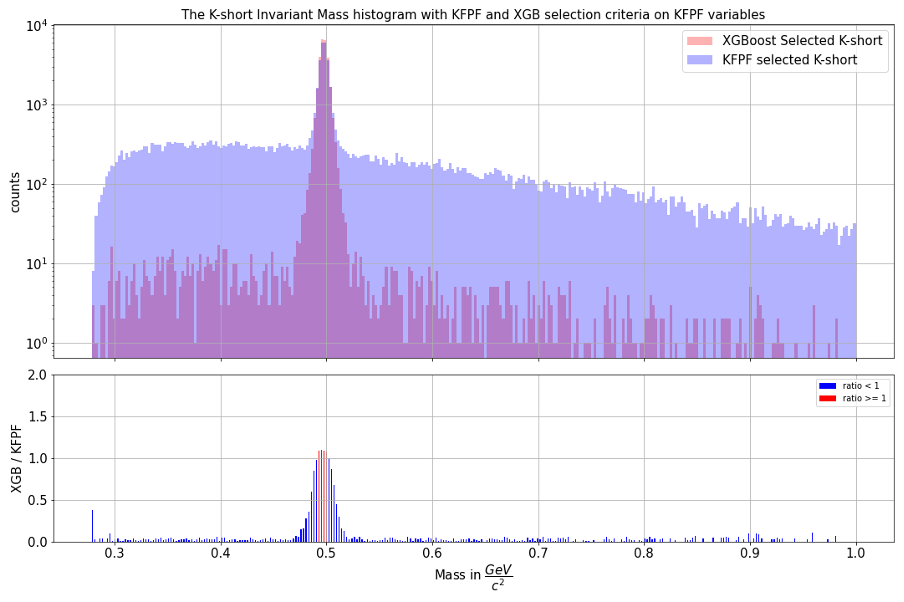
\includegraphics[width=\textwidth]{img/better_reduction1.png} 
        \caption{Invariant mass distribution (y log scale)} 
        \vspace{0.3cm}
    \end{subfigure}
     \hfill
       \begin{subfigure}[b]{0.99\linewidth}
        \centering
        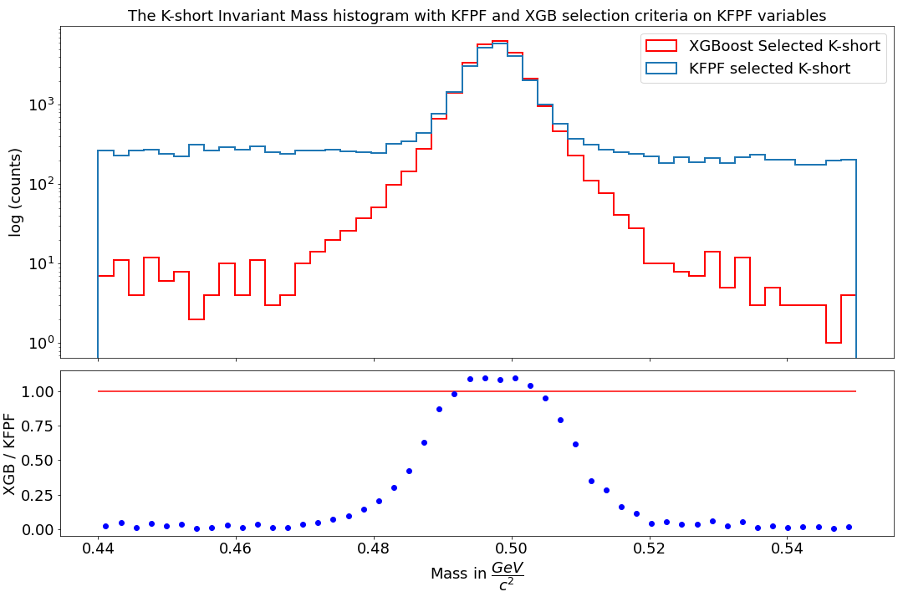
\includegraphics[width=\textwidth]{img/better_reduction2.png} 
        \caption{Invariant mass distribution (close-up)}
        \vspace{0.3cm}
    \end{subfigure}
    \caption{Comparison with KFPF cuts}\label{bckgr}
\end{figure}

With a cut value set to 0.86, we get $20\%$ better efficiency (Fig. \ref{effic}):
\begin{itemize}
    \item \textbf{Reconstructed \PKshort / reconstructible \PKshort = 95.91\%}  vs. 76.93\% with default KFPF cuts
    \item \textbf{false / true positive rate = 1.27} vs. 2.01 with default KFPF cuts
\end{itemize}
\begin{figure}
 \centering
    \begin{subfigure}[b]{0.99\linewidth} 
        \centering
        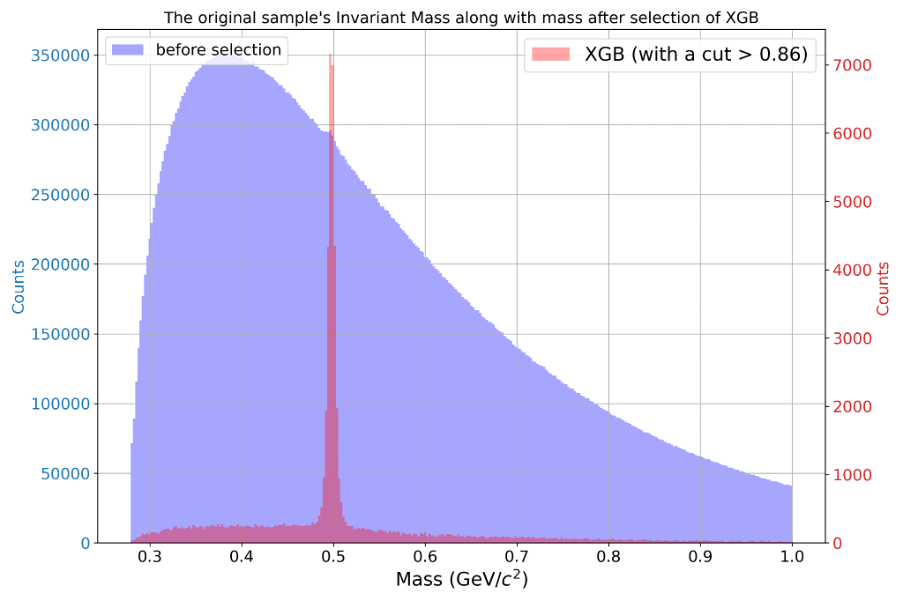
\includegraphics[width=\textwidth]{img/better_efficiency1.png} 
        \caption{Invariant mass distribution (y log scale)} 
        \vspace{0.3cm}
    \end{subfigure}
     \hfill
       \begin{subfigure}[b]{0.99\linewidth}
        \centering
        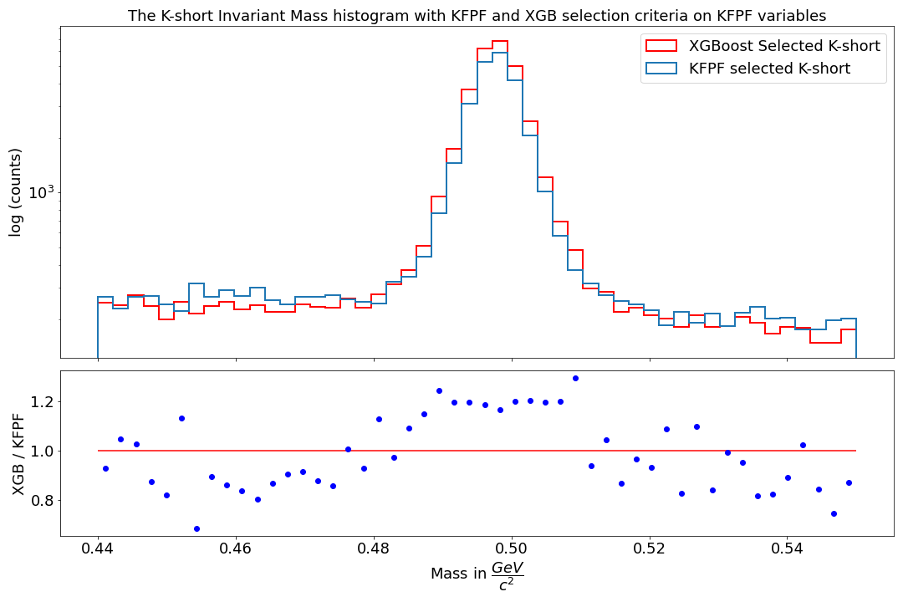
\includegraphics[width=\textwidth]{img/better_efficiency2.png} 
        \caption{Invariant mass distribution (close-up) - comparison with KFPF cuts}
        \vspace{0.3cm}
    \end{subfigure}
    \caption{Invariant mass distribution for probability $>$ 0.86}\label{effic}
\end{figure}

%--------------------- Investigation of potential bias
\subsubsection{Investigation of potential bias}
To check if the XGB selection criteria cut tails of the distribution, or are biased in some regions, the invariant mass distribution of true and false positives is plotted (Figure. \ref{true-false}).
\begin{figure}[h!]
 \centering
    \begin{subfigure}[b]{0.79\linewidth} 
        \centering
        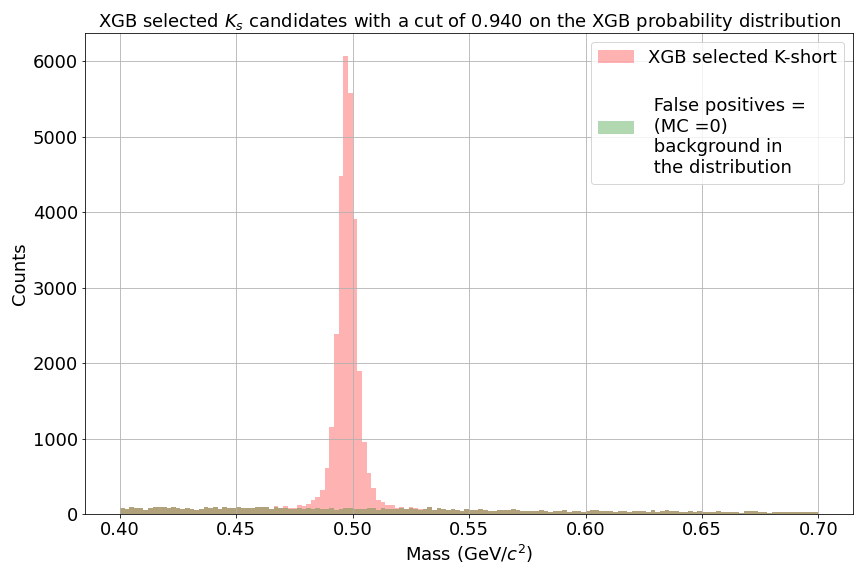
\includegraphics[width=\textwidth]{img/true_and_false_signal.png} 
        \caption{Selected \PKshort and false positives distribution} 
        \vspace{0.3cm}
    \end{subfigure}
     \hfill
       \begin{subfigure}[b]{0.69\linewidth}
        \centering
        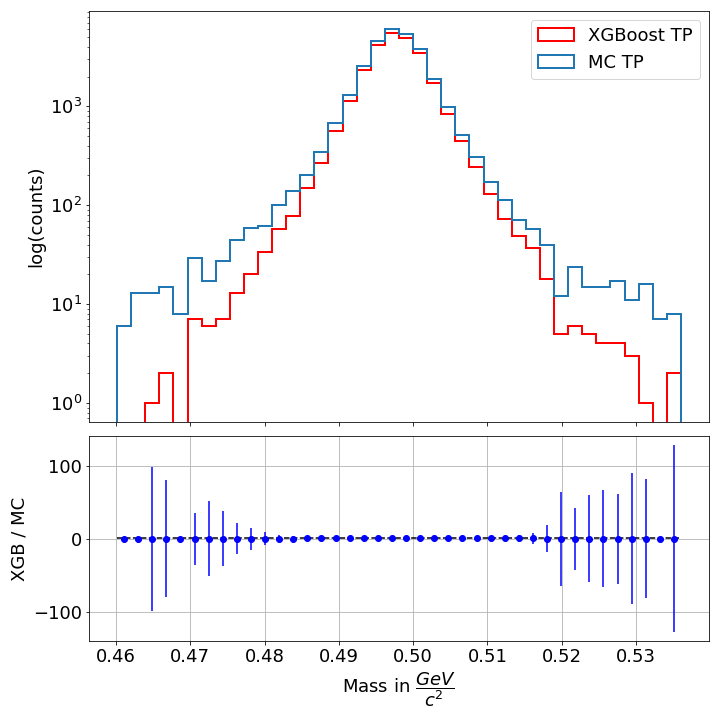
\includegraphics[width=\textwidth]{img/efficiency_plot_mass.png} 
        \caption{Reconstructed and MC true positives (y log scale)}
        \vspace{0.3cm}
    \end{subfigure}
    \caption{True-false positives investigation}
    \label{true-false}
\end{figure}
We see that our model does not seem to be biased towards any invariant mass region.

\newpage
%----------------------- results for 3.3A GeV/c
\subsection{Results for $p_{\text{beam}}$ = 3.3A GeV/c}

\subsubsection{Comparison with KFPF cuts}
The same code can be used to obtain similar results for another CBM energy level. Comparing to default KFPF cuts, with probability cut 0.9635 (Fig. \ref{33agev}):
\begin{itemize}
    \item \textbf{Reconstructed \PKshort / reconstructible \PKshort = 93.45\%}  vs. 78.94\% with default KFPF cuts
    \item \textbf{false / true positive rate = 0.19} vs. 1.38 with default KFPF cuts
\end{itemize}

\begin{figure}[h!]
 \centering
    \begin{subfigure}[b]{0.99\linewidth} 
        \centering
        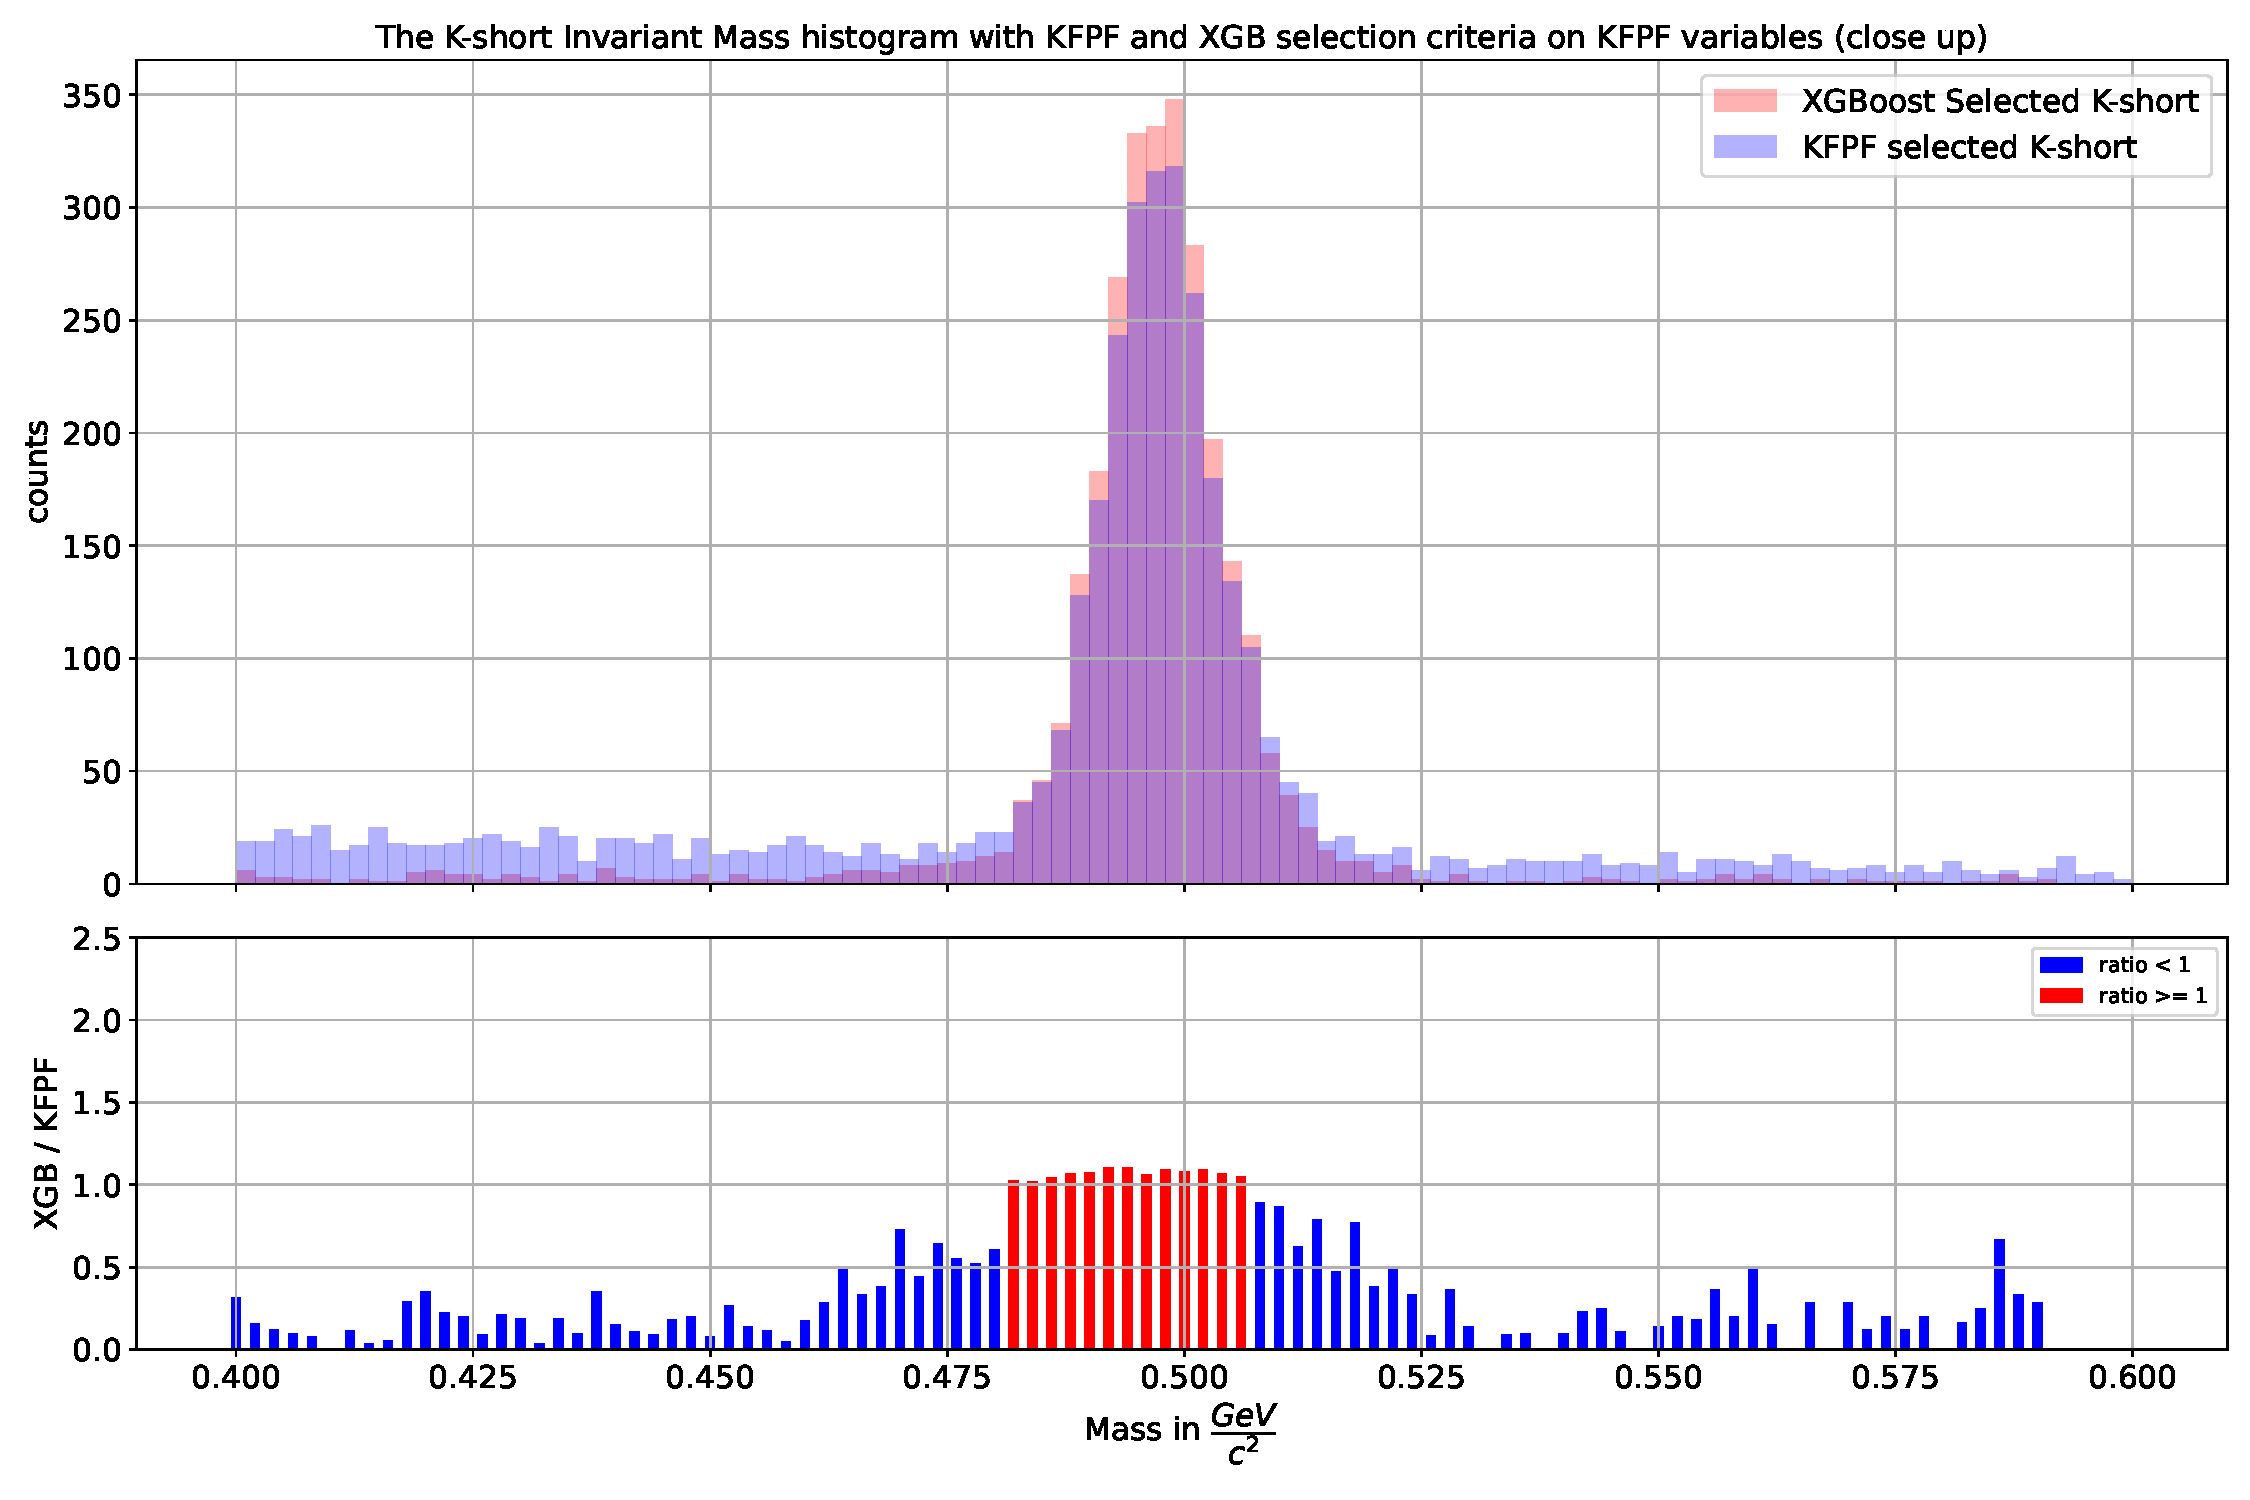
\includegraphics[width=\textwidth]{img/kaon_inv_mass_comparison_closeup.pdf} 
        \caption{Invariant mass distribution (y log scale)} 
        \vspace{0.3cm}
    \end{subfigure}
     \hfill
       \begin{subfigure}[b]{0.99\linewidth}
        \centering
        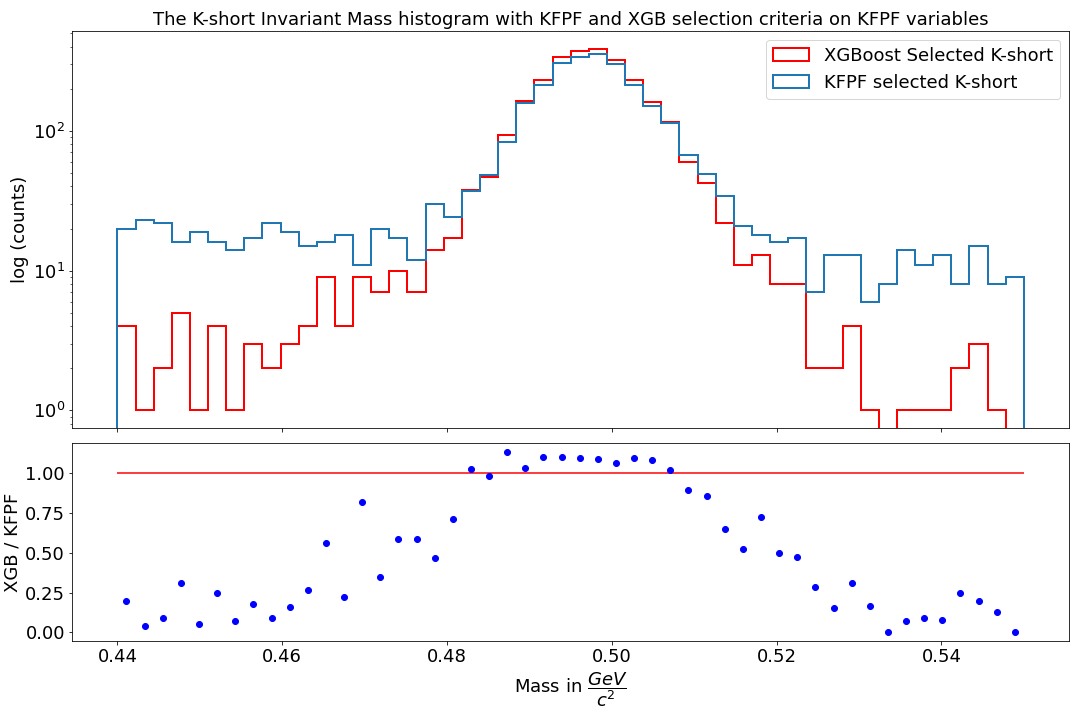
\includegraphics[width=\textwidth]{img/circle_kshort_invmass_with_ML.png} 
        \caption{Invariant mass distribution (close-up)}
        \vspace{0.3cm}
    \end{subfigure}
    \caption{Comparison with KFPF cuts for 3.3A GeV/c}\label{33agev}
\end{figure}
Due to the smaller statistics for this energy level, the ML model training should be redone for a bigger dataset.

%-------------- Influence of the magnetic field scaling
\subsection{Influence of the magnetic field scaling}
Obtained ML model can be adapted for the investigation of the influence of the magnetic field scaling. We compare: 100\% MF strength (for  $p_{\text{beam}}$ = 12A GeV/c), 56\% and 27.5\% MF strength (for $p_{\text{beam}}$ = 3.3A GeV/c, both with only DCM generated data for 0.4M events for training and 0.1M for validation). We see (Fig. \ref{mf}) that the stronger the magnetic field is, the broader \PKshort invariant mass distribution peak is. Also, we observe much more signal entries for $p_{\text{beam}}$ = 12A GeV/c (for the same number of events). \\

For $p_{\text{beam}}$ = 3.3A GeV/c the number of signal entries is almost the same; we select the probability cut so that the false/true positive ratio is the same for both \% of MF and compare the efficiency of the reconstruction (Tab. \ref{tab:mf}). We see that weaker MF does not necessarily worsen efficiency (only 2\% difference). However, this comparison should also be redone for a bigger dataset.

\begin{table}[h!]
\begin{tabular}{|l|l|l|l|}
\hline
\textbf{ratio} &
  \textbf{\begin{tabular}[c]{@{}l@{}}12 A GeV/c \\ MF=100\%\end{tabular}} &
  \textbf{\begin{tabular}[c]{@{}l@{}}3.3 A GeV/c \\ MF=56\%\end{tabular}} &
  \textbf{\begin{tabular}[c]{@{}l@{}}3.3 A GeV/c \\ MF=27.5\%\end{tabular}} \\ \hline
\begin{tabular}[c]{@{}l@{}}reconstructed/\\ reconstructible\end{tabular} &
  89.98\% &
  90.36\% &
  88.49\% \\ \hline
\begin{tabular}[c]{@{}l@{}}false / \\ true positive\end{tabular} &
  0.2 &
  0.2 &
  0.2 \\ \hline
\end{tabular}
\caption{\label{tab:mf}Comparison of MF strength vs. efficiency}
\end{table}

\begin{figure}[h!]
 \centering
    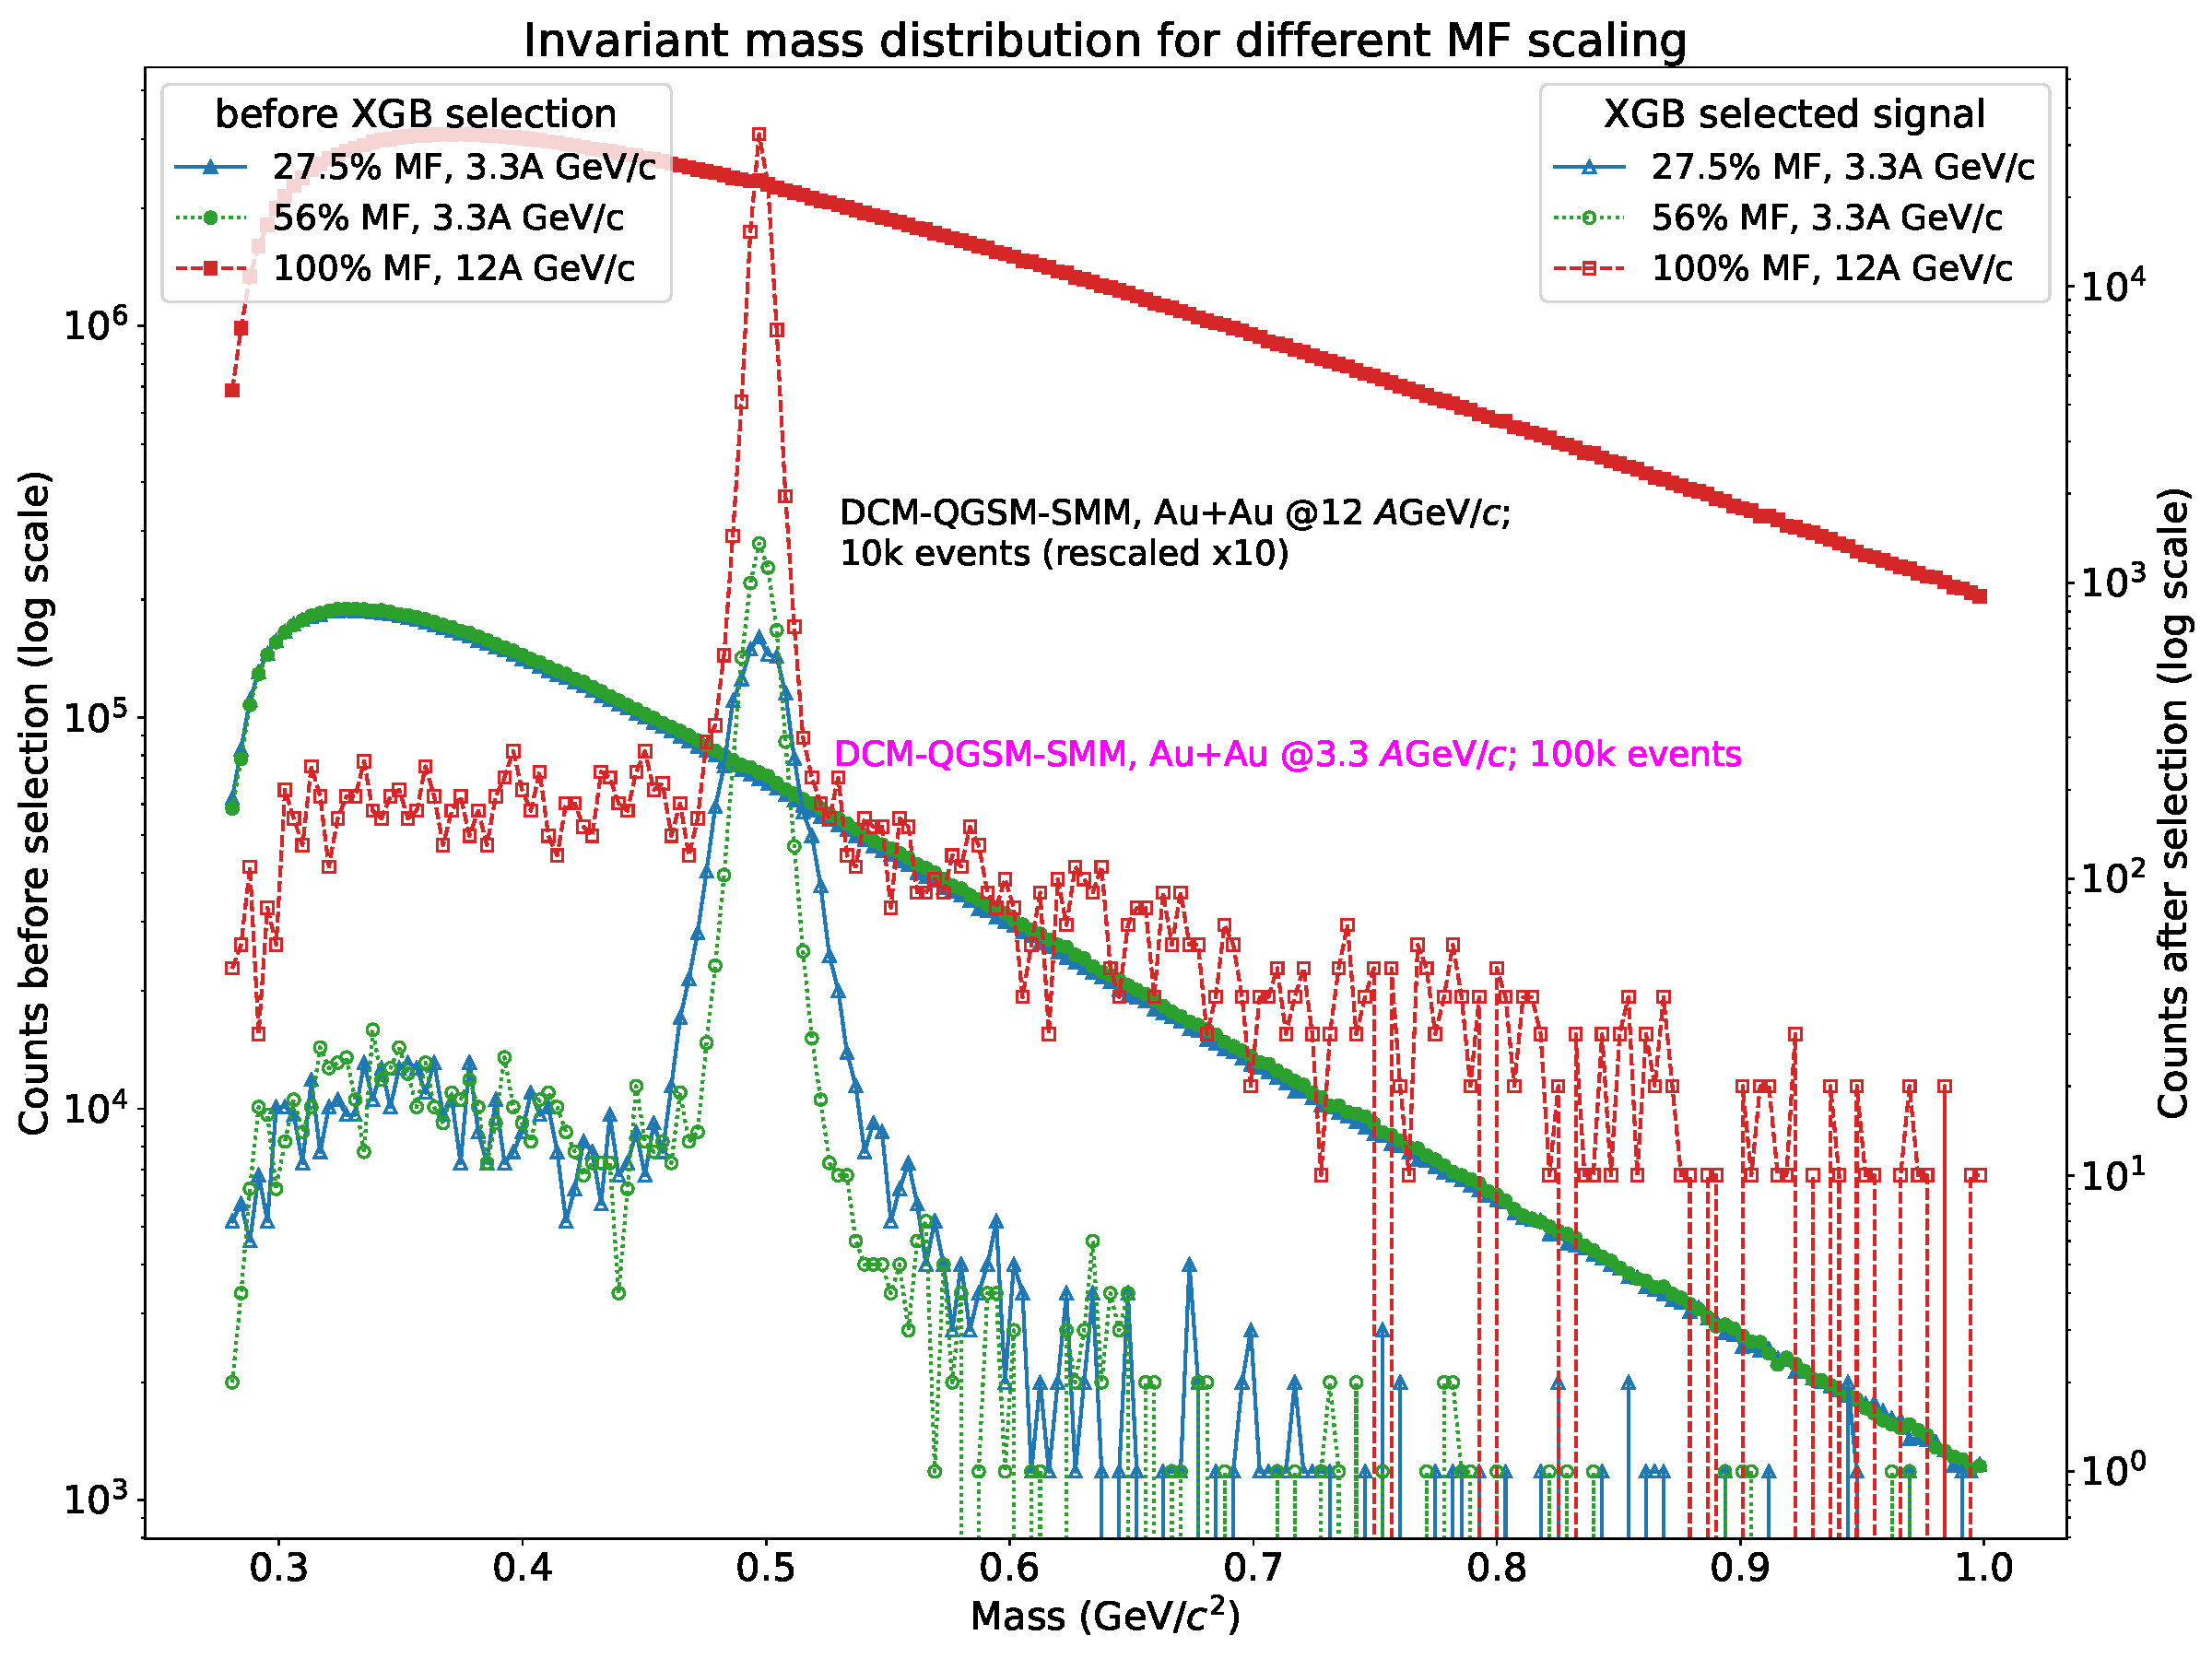
\includegraphics[width=\textwidth]{img/mf0log.pdf} 
    \vspace{0.1cm}
    \caption{Invariant mass distribution for different MF scaling}
    \label{mf}
\end{figure}


